%sample file for Modelica 2011 Abstract page

\documentclass[11pt,a4paper]{article}
\usepackage{graphicx}
% uncomment according to your operating system:
% ------------------------------------------------
\usepackage[latin1]{inputenc}    %% european characters can be used (Windows, old Linux)
%\usepackage[utf8]{inputenc}     %% european characters can be used (Linux)
%\usepackage[applemac]{inputenc} %% european characters can be used (Mac OS)
% ------------------------------------------------
\usepackage[T1]{fontenc}   %% get hyphenation and accented letters right
\usepackage{mathptmx}      %% use fitting times fonts also in formulas
% do not change these lines:
\pagestyle{empty}                %% no page numbers!
\usepackage[left=35mm, right=35mm, top=15mm, bottom=20mm, noheadfoot]{geometry}
%% please don't change geometry settings!
\usepackage{pgfplots}
\pdfminorversion=4

% begin the document
\begin{document}
\thispagestyle{empty}

\title{\textbf{Remarks on the Implementation of the Modelica Standard Tables}}
\author{Thomas Beutlich \quad Gerd Kurzbach \quad Uwe Schnabel\\
ITI GmbH\\
Schweriner Stra\ss{}e 1, 01067 Dresden, Germany\\
\{beutlich, kurzbach, schnabel\}@itisim.com}
\date{} % <--- leave date empty
\maketitle\thispagestyle{empty} %% <-- you need this for the first page

This article reveals some implementation details regarding the C code of the revised table interpolation blocks released with the Mod\-el\-ica Standard Library (MSL) 3.2.1. This new table implementation was named \emph{Mod\-el\-ica Standard Tables} and comprises the following four blocks for univariate and bivariate interpolation
\begin{itemize}
\item Mod\-el\-ica.Blocks.Sources.CombiTimeTable,
\item Mod\-el\-ica.Blocks.Tables.CombiTable1D,
\item Mod\-el\-ica.Blocks.Tables.CombiTable1Ds and
\item Mod\-el\-ica.Blocks.Tables.CombiTable2D.
\end{itemize}

The emphasis is placed on the unique features of the CombiTimeTable which are the discontinuities by time events and the periodic extrapolation (Fig.~\ref{fig:2e}). For instance, periodic and discontinuous signals like saw-tooth or square-wave w.r.t. simulation time can be modeled in a very convenient and compact way. However, the numerically stable detection of periodic time events is rather tricky since floating-point arithmetic must not be used to detect them.
\begin{figure}[!htbp]
\centering
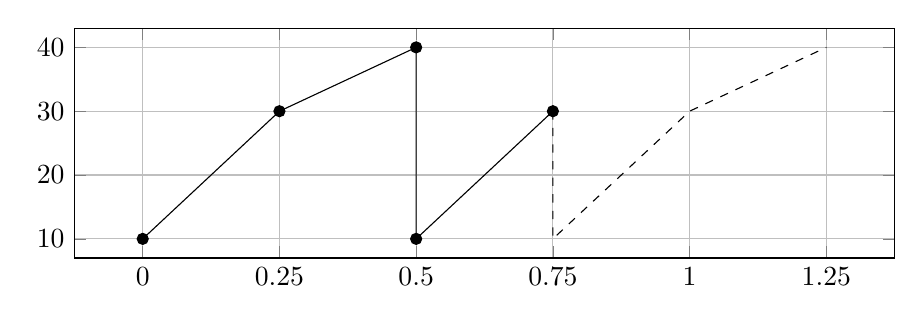
\begin{tikzpicture}
\begin{axis}[height=4.5cm, width=12cm, grid=major, enlargelimits=true, xtick={0,0.25,0.5,0.75,1,1.25}]
\addplot [mark=none] coordinates {
(0,10)
(0.25,30)
(0.5,40)
(0.5,10)
(0.75,30)
};
\addplot [mark=none, style=dashed] coordinates {
(0.75,30)
(0.75,10)
(1,30)
(1.25,40)
};
\addplot [only marks,mark=*] coordinates {
(0,10)
(0.25,30)
(0.5,40)
(0.5,10)
(0.75,30)
};
\end{axis}
\end{tikzpicture}
\caption{There are two time events per period in case of linear interpolation and periodic extrapolation of the 5$\times$2 time table $[$0, 10; 0.25, 30; 0.5, 40; 0.5, 10; 0.75, 30$]$.}
\label{fig:2e}
\end{figure}

Besides the CombiTimeTable basic information on the univariate and bivariate interpolation by Akima splines~\cite{Akima:1970:NMI:321607.321609, Akima:1974:MBI:360767.360779} and the available table array memory optimization options are summarized. Last but not least, the remaining newly implemented table interpolation features are also mentioned.

\begin{thebibliography}{00}
\addcontentsline{toc}{chapter}{References}

\bibitem{Akima:1970:NMI:321607.321609}
Hiroshi Akima.
\newblock A new method of interpolation and smooth curve fitting based on local
  procedures.
\newblock {\em J. ACM}, 17(4):589--602, October 1970.

\bibitem{Akima:1974:MBI:360767.360779}
Hiroshi Akima.
\newblock A method of bivariate interpolation and smooth surface fitting based
  on local procedures.
\newblock {\em Commun. ACM}, 17(1):18--20, January 1974.

\end{thebibliography}

\end{document}
